
\chapter{Search Strategy}
\label{ch:SearchStrategy}
%Deep thoughts go here.
This chapter contains co-authored material from Ref.~\cite{Dijet2017}, written as part of the ATLAS Collaboration.
\newline

Compared to most ATLAS analyses, the search strategy is very straightforward:

\begin{itemize}[noitemsep]
	\item Event passes the lowest unprescaled trigger, HLT\_j380
	\item Events are part of the Good Run List
	\item Events are not flagged as having a calorimeter noise burst, or as having incomplete event data
	\item Leading jet $\pt > 440$\,GeV
	\item Subleading jet $\pt > 60$\,GeV
	\item All jets with $\pt > 60$\,GeV pass jet cleaning cuts
\end{itemize}

To help discriminate between the $t$-channel dominated QCD background and any possible $s$-channel resonances from new physics processes, a cut is placed on the angular variable
\begin{equation}
y^* = \frac{y_1 + y_2}{2}
\end{equation}
where $y_1$ and $y_2$ are the rapidities of the leading and subleading jets, respectively.  The cut is chosen as it has the best discrimination between signal and background for the ensemble of benchmark models used, or for the single benchmark in the case of the $W^*$ selection.  Finally, a cut is placed on the invariant mass of the two leading jets to ensure that the trigger is fully efficient when paired with the $y^*$ cut.  The cuts for the resonance and $W^*$ resonance selections are:

\begin{itemize}[noitemsep]
	\item $|y^*| <$ 0.6 (1.2)
	\item $\mjj >$ 1.1 (1.7)\,TeV
\end{itemize}



\section{Background Fit}
Previous versions of the dijet resonance analysis, including those from CDF, ATLAS, and CMS, have fit the dijet invariant mass spectrum with a function of the form
\begin{equation}
f(z) = p_1(1-z)^{p_2}z^{p_3+p_4 ln(x)+p_5 ln(x)^2}
\label{eq:dijet}
\end{equation}
where $z = m_{jj}/\sqrt{s}$ and the behavior is governed by the free parameters $p_i$.  Some past searches have required fewer terms in Eq.~\ref{eq:dijet}, such as by setting $p_4 = p_5 = 0$, but more parameters are required to properly describe the distribution as integrated luminosity increases.  Eq.~\ref{eq:dijet} was found to fit the observed spectrum in searches at CDF, and in ATLAS and CMS searches at both $\sqrt{s}$ = 8 and $\sqrt{s}$ = 13\,TeV.  The parameterization also fits the distribution obtained from simulated QCD samples.

For the analysis of the full 2015+2016 ATLAS dataset, there was a worry that the aforementioned function would no longer be sufficient to properly describe the dataset.  While additional parameters could be added to Eq.~\ref{eq:dijet}, the function is already ad-hoc in nature, and any additional terms could possibly see diminishing returns in usefulness.  As such, this analysis was used to test and implement a new method for fitting the background, resulting in the use of the sliding-window fit, or SWiFt as the specific implementation was named.  The goal was to create a fitting method that was more robust against increases in luminosity while maintaining the same results in the regime where the global fit still held.

\subsection{The Wilks' Statistical Test}

To ensure that enough parameters are included in the fit function used to properly describe the observed spectrum, it must be determined that adding additional terms does not significantly improve the fit, and that any bumps in the observed spectrum do not come from under-fitting the data.  To determine the number of parameters needed, the Wilks' statistic is used.  When comparing lower and higher parameter versions of Eq.~\ref{eq:dijet}, the statistic reveals how much of an improvement an additional parameter in the fit function provides.  In the case of a p-value$<$0.05, the $n-1$ parameter function is discarded, and the statistic for $n$ vs. $n+1$ is calculated.  The evolution of the test statistics over time is shown in Figure~\ref{fig:Wilks}.  For the full 37\,fb$^{-1}$ dataset the 4-parameter function is preferred.  The decline in the viability of the 3-parameter function is clearly visible, becoming unviable once around 25\,fb$^{-1}$ of data is used.

\begin{figure}[h!]
	\centering
	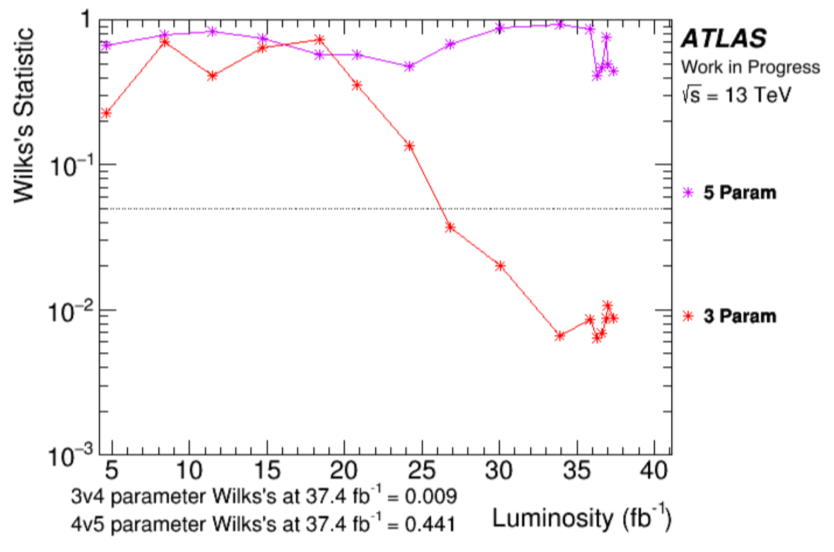
\includegraphics[width=0.75\columnwidth]{figures/SearchStrategy/Wilks.png}
	\caption{Wilks' test between the 4-parameter fit function and the 3/5-parameter versions.  For the full 2015+2016 dataset, the 4-parameter fit provides a much better description of the data than the 3-parameter fit, but the 5-parameter fit does not provide additional improvement.}
	\label{fig:Wilks}
\end{figure}

For the full dataset, a global fit function with four parameters is still a viable fit.  (If a 5-parameter version was preferred, a 6th parameter would be needed to assess the goodness of fit, but such a term has not yet been determined)  This means that a direct comparison can be made between the sliding window fit and the global fit to ensure that the sliding window gives the same results.

\subsection{The Sliding Window Fit (SWiFt)}

The nominal size for the sliding window was chosen as the largest window which used one less parameter than the global fit while still proving a good fit to the function for all possible windows.  The three metrics used to measure this were the Wilks' statistic, chi-squared divided by the number of degrees of freedom, and the Kolmogorov-Smirnov (KS) test.  The results for various window sizes are show in Figure~\ref{fig:SwiftFitStats}.  All of the tested windows performed very well with the data, but the final chosen window uses 30 bins to the left of the center and 20 bins to the right, comprising approximately half of the total distribution, and larger than any of the tested signal shapes.  The asymmetry in the window allows for a stronger contribution from the higher-statistics, low-\mjj~bins in a given window to better anchor the fit as the window slides to the tail of the distribution.

\begin{figure}[ht!]
	\centering
	\subfloat[]{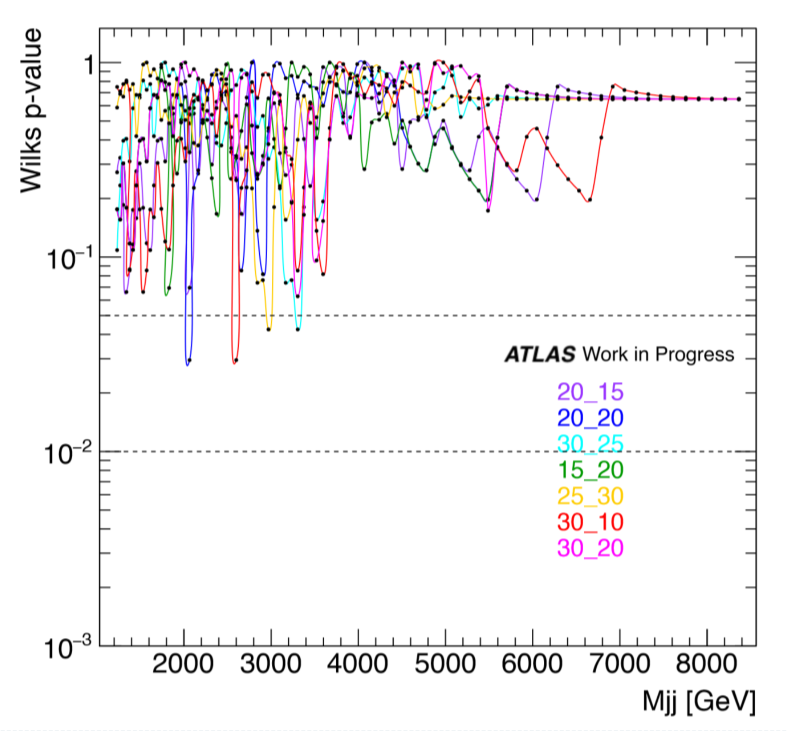
\includegraphics[width=0.45\columnwidth]{figures/SearchStrategy/SwiftWilks.png}\label{subfig:SwiftWilks}}
	\hspace{0.1\textwidth}%
	\subfloat[]{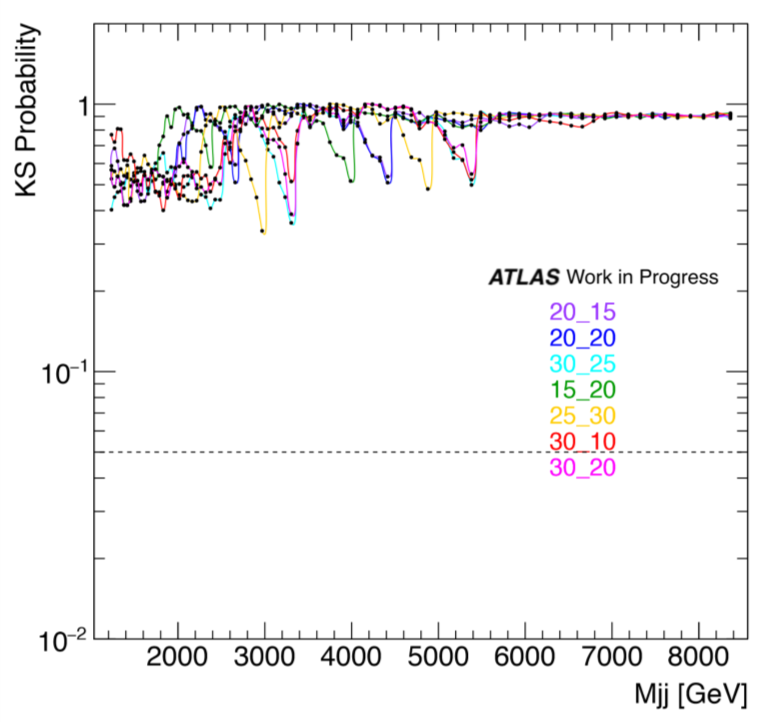
\includegraphics[width=0.45\columnwidth]{figures/SearchStrategy/SwiftKS.png}\label{subfig:SwiftKS}}
	\subfloat[]{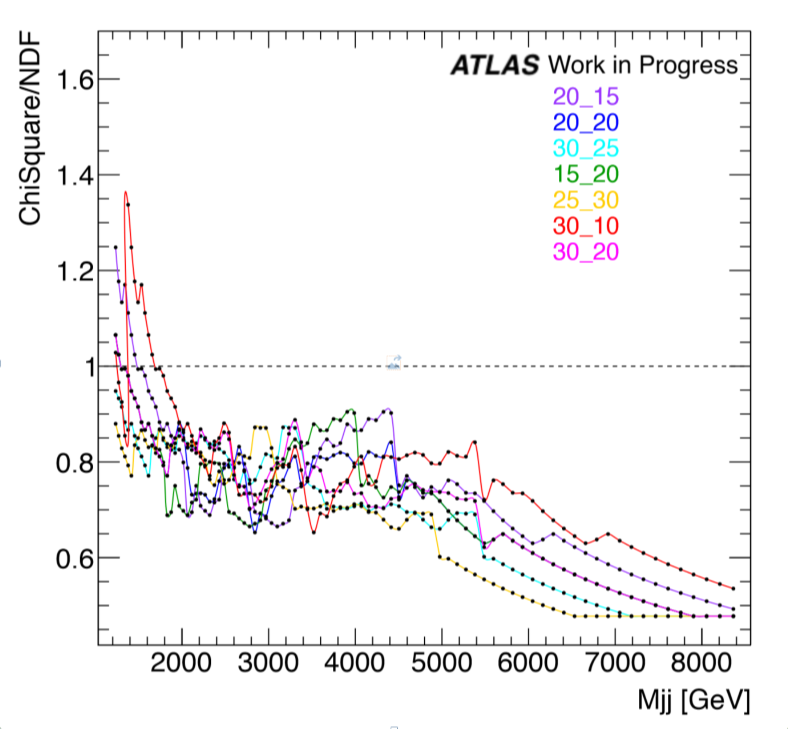
\includegraphics[width=0.45\columnwidth]{figures/SearchStrategy/SwiftChi2.png}\label{subfig:SwiftChi2}}
	\caption{Statistical measures used to determine the optimal window size for SWift. (a) Wilks' p-value comparing the nominal SWiFt 3-parameter fit with an alternate 4-parameter version (b) KS p-value comparing the fit to pseudodata (c) $\chi^2$/NDF comparing fit to pseudodata. }
	\label{fig:SwiftFitStats}
\end{figure}

For each window, a fit is performed to the bins in the window using the three-parameter form of Eq.~\ref{eq:dijet}. The fit is used to give a background value at the bin "center" (keeping in mind that the window is asymmetric), and the center then slides one bin to the right and creates the next fit and returns a value for the next bin center.  This is done across the entire spectrum, including beyond the final filled bin in the data distribution.  The values for each center are then stitched together to create the full background distribution.

To ensure the best fit across the whole spectrum, the sliding window changes shape at the two extremes of the distribution.  As it approaches the end of the distribution at low \mjj, the left side of the window is compressed down, shrinking to a smallest size of 10 bins to the left, 20 bins to the right.  This does not cause any loss in efficacy as the window fit is relatively insensitive to window size, as demonstrated by the 15\_20 window line in Figure~\ref{fig:SwiftFitStats}.  Below this point in the spectrum, the fit value for all bins below the window center is determined by their fit in this smallest window.  At the high-\mjj~end, the left side of the window is fixed once the window center reaches the 5.5\,TeV bin, and past that point the window expands in size.  This is done to maintain adequate statistics in the fit, especially as the window slides beyond the end of the data spectrum.  This system is demonstrated in Figure~\ref{fig:SwiftSlide}.

\begin{figure}[]
	\centering
	\subfloat[]{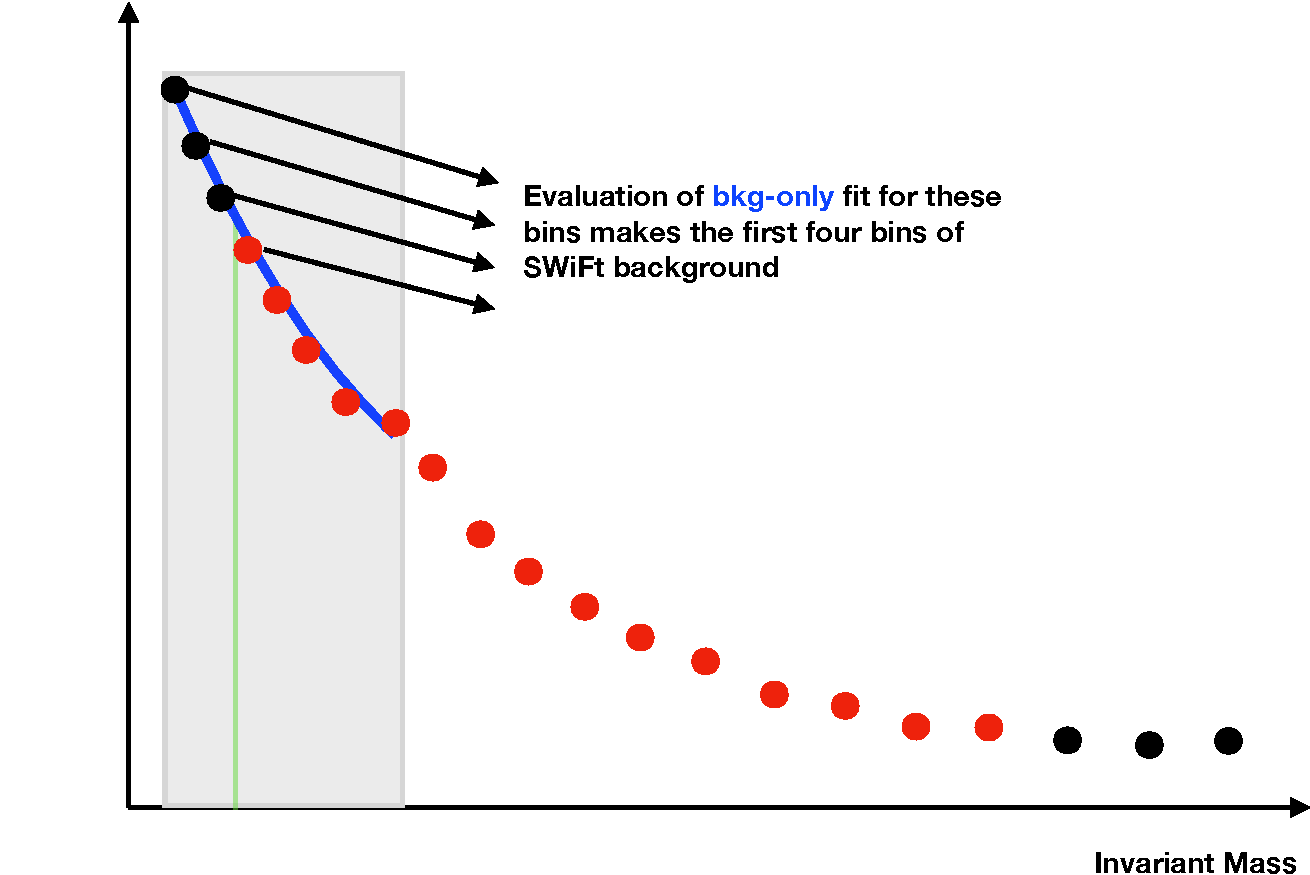
\includegraphics[width=0.45\columnwidth]{figures/SearchStrategy/SwiftSlide1.pdf}\label{subfig:SwiftSlide1}}
	\subfloat[]{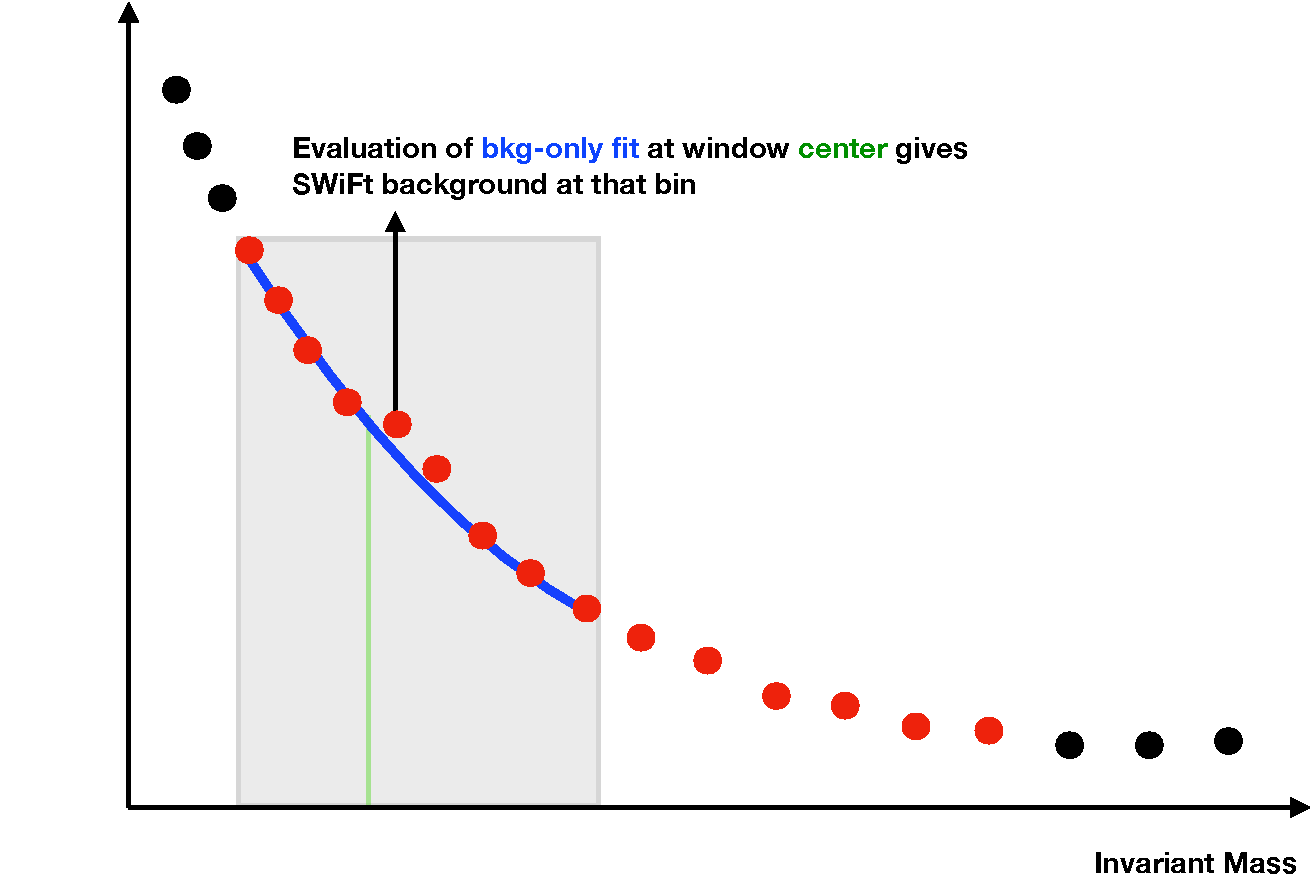
\includegraphics[width=0.45\columnwidth]{figures/SearchStrategy/SwiftSlide2.pdf}\label{subfig:SwiftSlide2}}
	\hspace{0.1\textwidth}%
	\subfloat[]{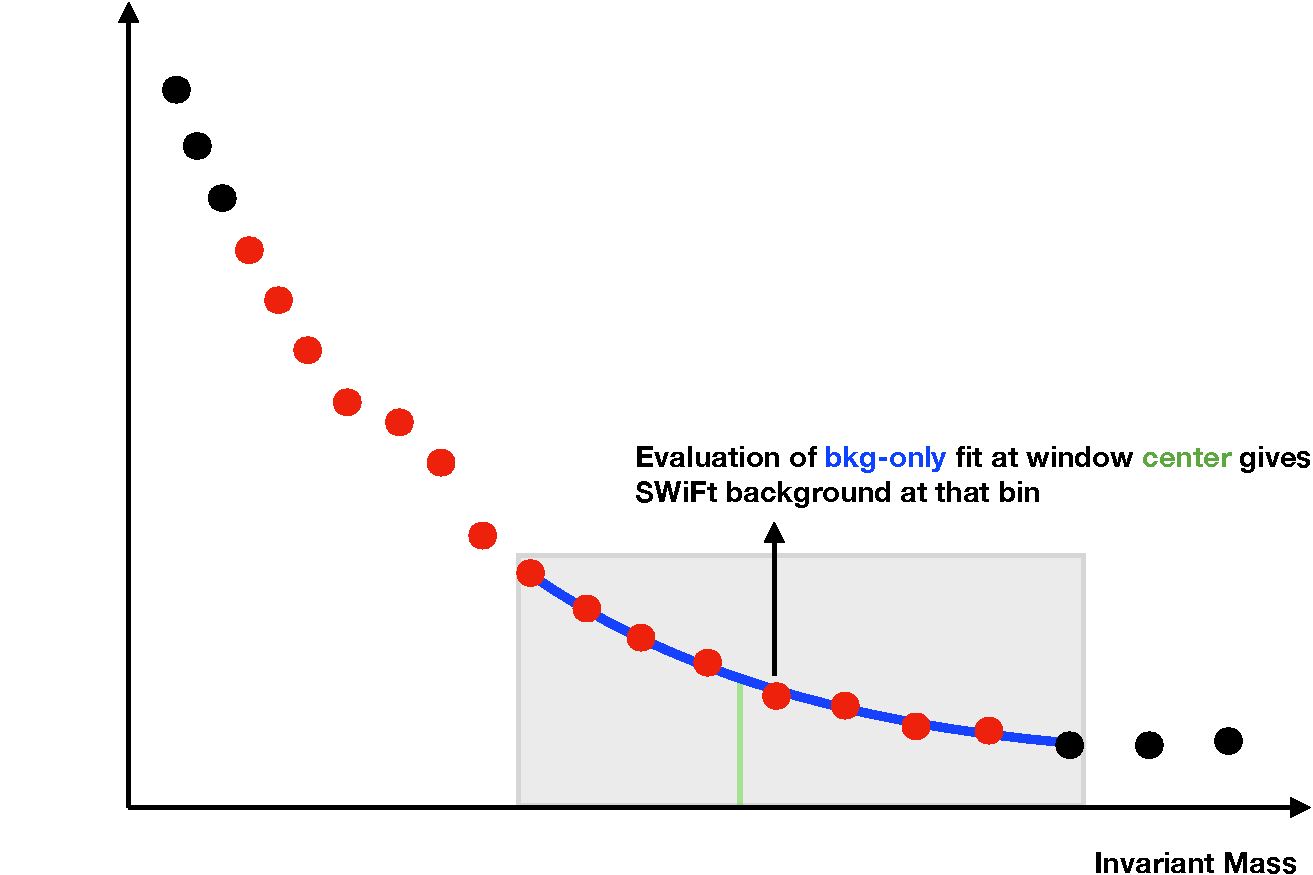
\includegraphics[width=0.45\columnwidth]{figures/SearchStrategy/SwiftSlide3.pdf}\label{subfig:SwiftSlide3}}
	\subfloat[]{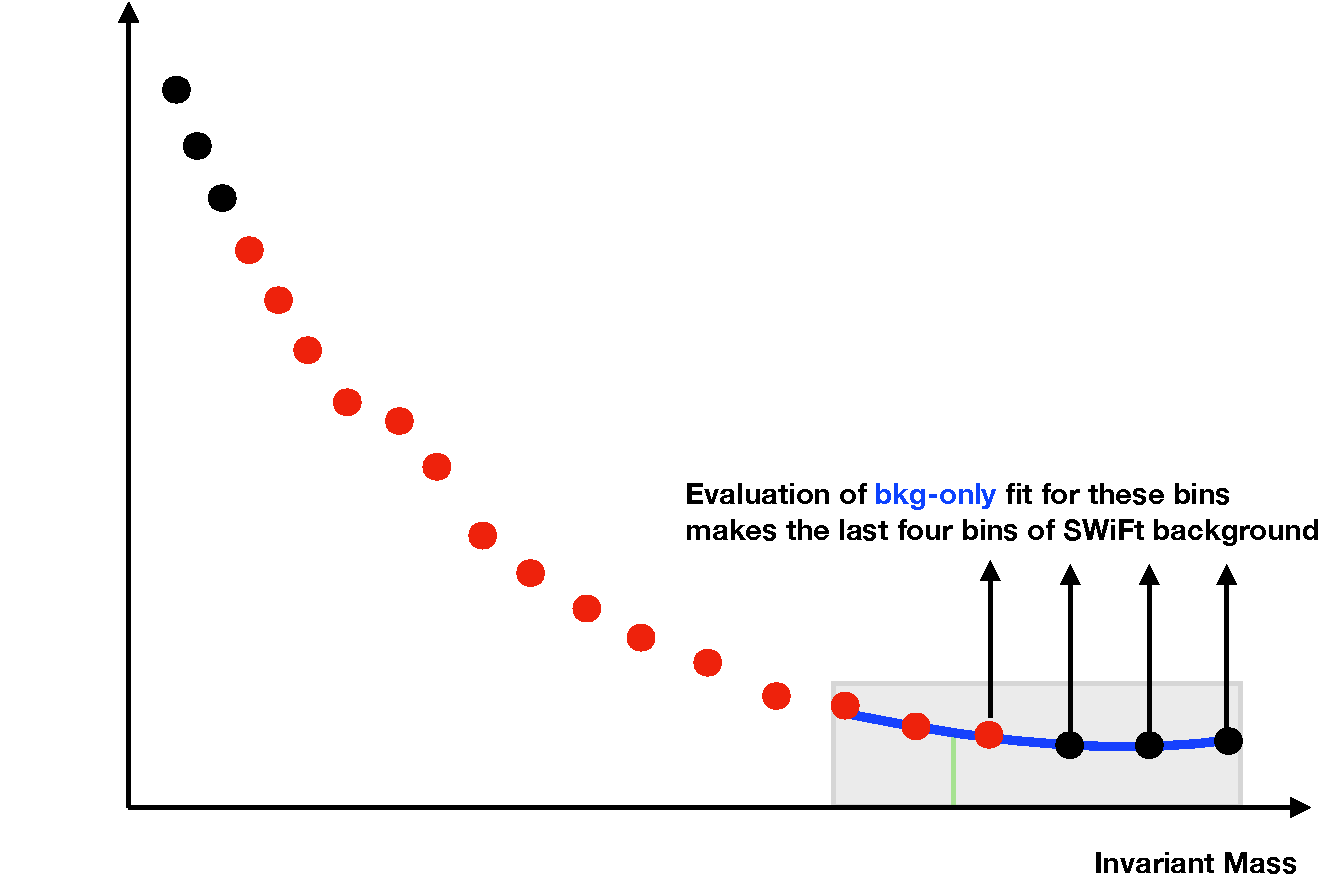
\includegraphics[width=0.45\columnwidth]{figures/SearchStrategy/SwiftSlide4.pdf}\label{subfig:SwiftSlide4}}
	\caption{An example of the bin-by-bin construction of the SWiFt background as seen in Ref.~\cite{SWiFt}.  The gray box shows the window considered at each point while the green line is the bin center for which the fit value is evaluated.  In (b) and (c) only the value at the bin center is used for the total background estimate, while in (a) and (d) the fit values before and after the center, respectively, are used as part of the overall background.}
	\label{fig:SwiftSlide}
\end{figure}

Figure~\ref{fig:SwiftVsGlobal} shows a comparison of the background obtained from SWiFt with the 4-parameter global fit function.  Across the full spectrum no significant deviations are observed, and the limits obtained using the two different background fits are essentially identical.  For the paper results, only the SWiFt background results are shown to prevent any confusion between the two methods, and to encourage future use of the SWiFt method for similar searches.

The full SWiFt method is now outlined in Ref.~\cite{SWiFt}, though it has evolved somewhat from its original implementation in the dijet search to its current form for use in future searches.

\begin{figure}[h!]
	\centering
	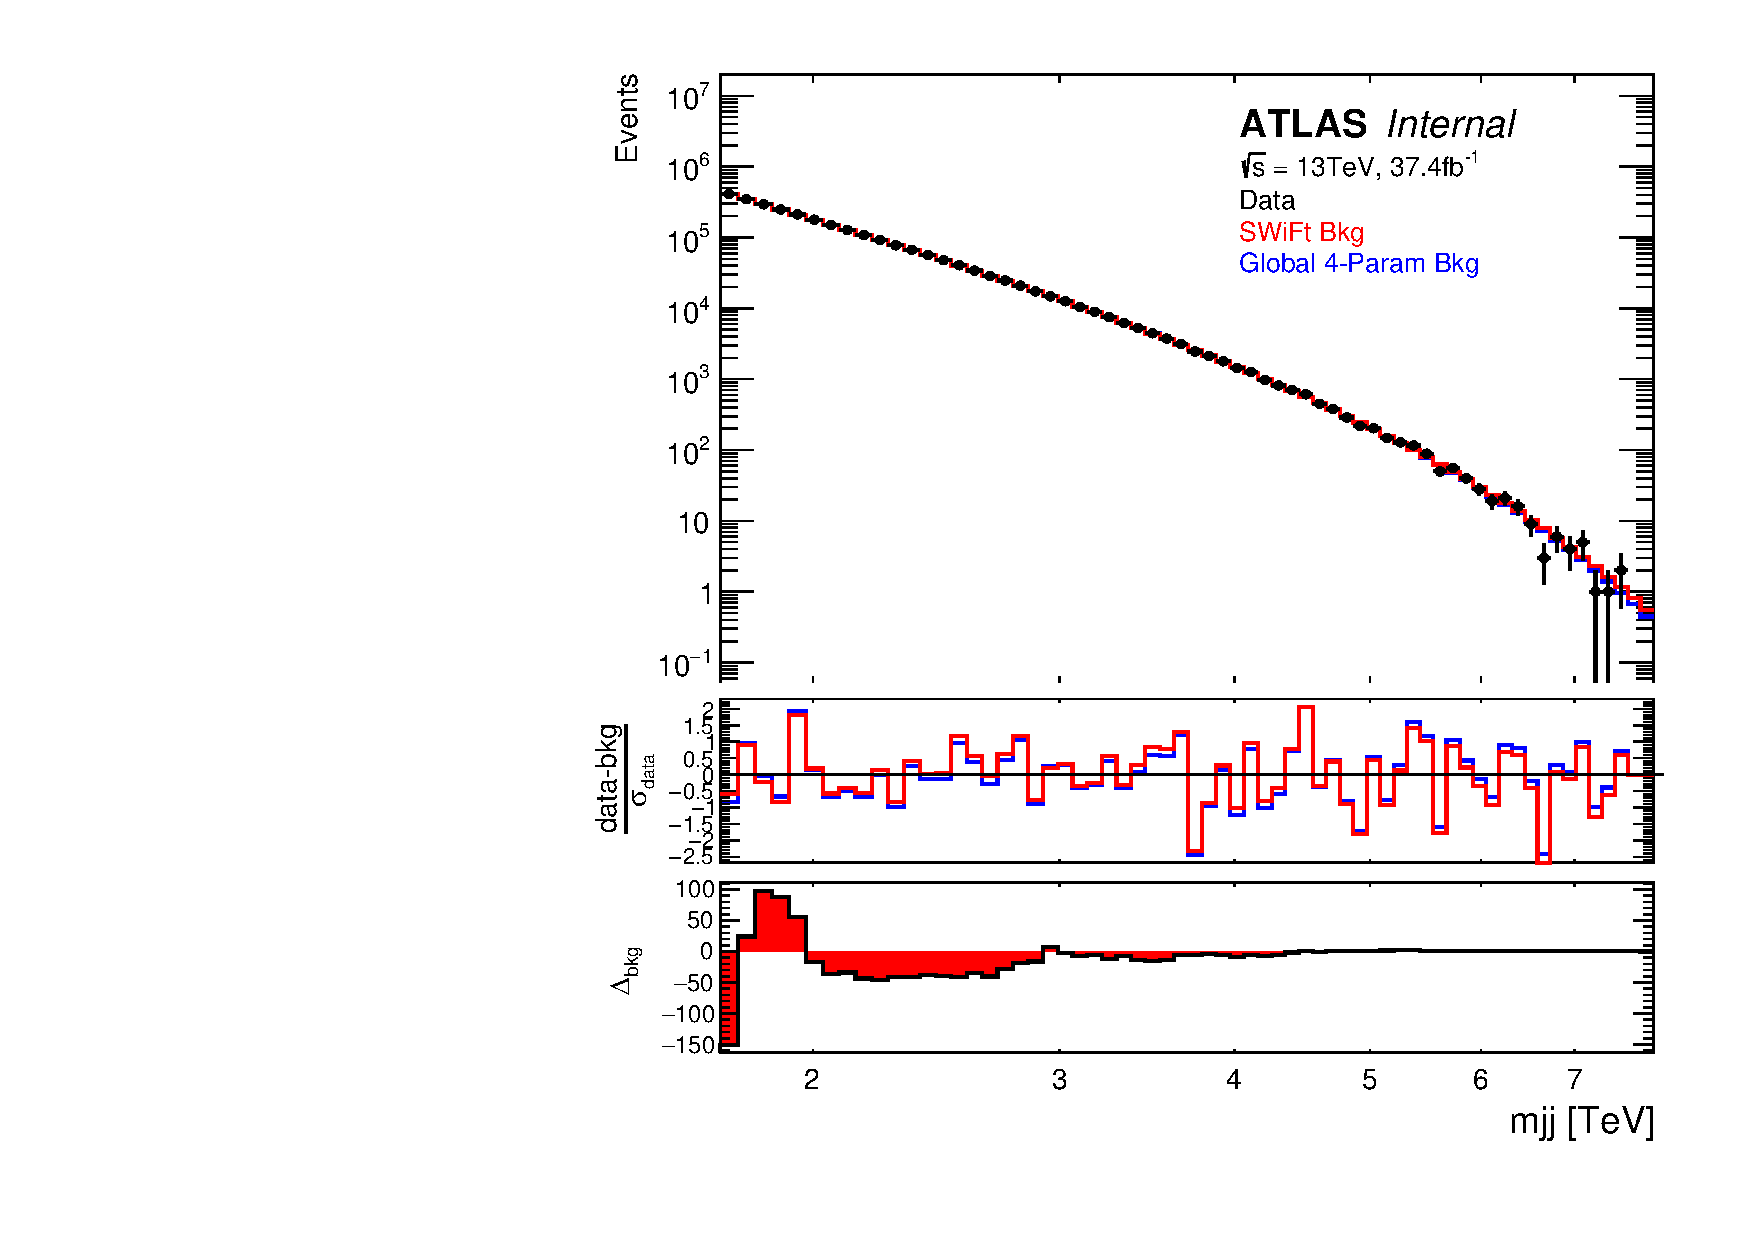
\includegraphics[width=0.75\columnwidth]{figures/SearchStrategy/SwiftVsGlobal.png}
	\caption{Comparison of the global 4-parameter fit function to the SWiFt background using a 3-parameter fit in each window.  No significant variations between the two fits are observed.}
	\label{fig:SwiftVsGlobal}
\end{figure}

\section{Search Phase}

The search phase of the analysis deals with determining if there are any signs of new physics in the data set.  In contrast to the previous fitting section which sought to address whether or not a better description of the data was available through a more complex fit function, the search phase asks whether or not the obtained fit and the actual data spectrum are consistent with each other.  The dijet analysis uses BumpHunter to create its test statistic as it insensitive to the shape of any possible excess.

\subsection{BumpHunter}

Statistical tests such as the $\chi^2$ test measure the discrepancy between data and expectation in a bin-by-bin basis, but do not take into account the relation between bins.  For example, five consecutive bins with excesses over background is much more interesting for a physics search than if those bins had the same significance but alternated signs between bins.  To look for the "bumpiness" of data compared to prediction, BumpHunter scans over sets of adjacent bins and measures the significance if those bins were combined together into one.  The dijet analysis scans for all possible combinations of bins from 2 bins to half the full spectrum, much wider than any of the signal templates considered in the analysis and certain to cover any possible cases of interest.  (Since the bin widths are chosen to approximate the detector resolution, a resonance creating an excess in only one bin is exceedingly unlikely)  From this scan BumpHunter returns the most discrepant region, identified in this search as the region 4326–4595\,GeV.

The global significance of the region is calculated by running BumpHunter over a set of 10,000 pseudo-experiments.  In each pseudo-experiment, a toy spectrum is created by Poisson-fluctuating each bin of the spectrum and then calcuating the BumpHunter test statistic for that toy.  From this set it is possible to calculate the portion of pseudo-experiments in which the observed data has an excess that is less significant.

For this particular search an excess was not observed, but it is worth noting the procedure that was in place for such an eventuality.  In the case that BumpHunter returned a most discrepant region with a p-value $<$ 0.01, representing a very significant excess, the background fit would be re-derived using the sliding window method with all bins in the discrepant region removed from the fit, in turn removing any bias in the fit caused by the large fluctuation.  This new fit would then be used as the background estimate for the limit setting phase.